\documentclass[twoside]{article}
\setlength{\oddsidemargin}{0.25 in}
\setlength{\evensidemargin}{-0.25 in}
\setlength{\topmargin}{-0.6 in}
\setlength{\textwidth}{6.5 in}
\setlength{\textheight}{8.5 in}
\setlength{\headsep}{0.75 in}
\setlength{\parindent}{0 in}
\setlength{\parskip}{0.1 in}


\usepackage{color}
\usepackage[pdftex]{graphicx}
\usepackage{sidecap}
\usepackage{wrapfig}
\usepackage{marvosym,url,hyperref}
%\usepackage{algorithm}
%\usepackage{algorithmic}
\usepackage{amsmath,amsfonts,graphicx}

%
% The following commands set up the lecnum (lecture number)
% counter and make various numbering schemes work relative
% to the lecture number.
%
\newcommand{\field}[1]{\mathbb{#1}} % requires amsfonts

\newcounter{lecnum}
\renewcommand{\thepage}{\thelecnum-\arabic{page}}
\renewcommand{\thesection}{\thelecnum.\arabic{section}}
\renewcommand{\theequation}{\thelecnum.\arabic{equation}}
\renewcommand{\thefigure}{\thelecnum.\arabic{figure}}
\renewcommand{\thetable}{\thelecnum.\arabic{table}}

%
% The following macro is used to generate the header.
%
\newcommand{\lecture}[4]{
   \pagestyle{myheadings}
   \thispagestyle{plain}
   \newpage
   \setcounter{lecnum}{#1}
   \setcounter{page}{1}
   \noindent
   \begin{center}
   \framebox{
      \vbox{\vspace{2mm}
    \hbox to 6.28in { {\bf C284r: Social Data Mining
	\hfill Fall 2015} }
       \vspace{4mm}
       \hbox to 6.28in { {\Large \hfill Lecture #1: #2  \hfill} }
       \vspace{2mm}
       \hbox to 6.28in { {\it Lecturer: #3 \hfill  #4} }
      \vspace{2mm}}
   }
   \end{center}
   \markboth{Lecture #1: #2}{Lecture #1: #2}

 
}
%
% Convention for citations is authors' initials followed by the year.
% For example, to cite a paper by Leighton and Maggs you would type
% \cite{LM89}, and to cite a paper by Strassen you would type \cite{S69}.
% (To avoid bibliography problems, for now we redefine the \cite command.)
% Also commands that create a suitable format for the reference list.
%\renewcommand{\cite}[1]{[#1]}
\def\beginrefs{\begin{list}%
        {[\arabic{equation}]}{\usecounter{equation}
         \setlength{\leftmargin}{2.0truecm}\setlength{\labelsep}{0.4truecm}%
         \setlength{\labelwidth}{1.6truecm}}}
\def\endrefs{\end{list}}
\def\bibentry#1{\item[\hbox{[#1]}]}

%Use this command for a figure; it puts a figure in wherever you want it.
%usage: \fig{NUMBER}{SPACE-IN-INCHES}{CAPTION}
\newcommand{\fig}[3]{
			\vspace{#2}
			\begin{center}
			Figure \thelecnum.#1:~#3
			\end{center}
	}
% Use these for theorems, lemmas, proofs, etc.
\newtheorem{theorem}{Theorem}[lecnum]
\newtheorem{lemma}[theorem]{Lemma}
\newtheorem{proposition}[theorem]{Proposition}
\newtheorem{claim}[theorem]{Claim}
\newtheorem{corollary}[theorem]{Corollary}
\newtheorem{definition}[theorem]{Definition}
\newtheorem{fact}[theorem]{Fact}
\newenvironment{proof}{{\bf Proof:}}{\hfill\rule{2mm}{2mm}}

% **** IF YOU WANT TO DEFINE ADDITIONAL MACROS FOR YOURSELF, PUT THEM HERE:

\newcommand\E{\mathbb{E}}


%%%%%%%%%%%%
%% colors %%
%%%%%%%%%%%%

\definecolor{MyBrick}{rgb}{0.9,0.00,0.00}
\newcommand\txtbrick[1]{{\color{MyBrick}{#1}}}

\definecolor{MyRed}{rgb}{0.99,0.00,0.00}
\newcommand\txtred[1]{{\color{MyRed}{#1}}}

\definecolor{MyWhite}{rgb}{1.00,1.00,1.00}
\newcommand\txtwhite[1]{{\color{MyWhite}{#1}}}

\definecolor{MyBlack}{rgb}{0.00,0.00,0.00}
\newcommand\txtblack[1]{{\color{MyBlack}{#1}}}

\definecolor{MyYellow}{rgb}{1.00,1.00,0.00}
\newcommand\txtyellow[1]{{\color{MyYellow}{#1}}}

\definecolor{MyDarkOrange}{rgb}{0.90,0.547,0.00}
\newcommand\txtorange[1]{{\color{MyDarkOrange}{#1}}}

\definecolor{MyOliveGreen}{rgb}{0.33,0.60,0.17}
\newcommand\txtgreen[1]{{\color{MyOliveGreen}{#1}}}

\definecolor{MyDarkMagenta}{rgb}{0.54,0.00,0.54}
\newcommand\txtmagenta[1]{{\color{MyDarkMagenta}{#1}}}

\definecolor{MyBrown}{rgb}{0.60,0.30,0.00}
\newcommand\colorcite[1]{{\color{MyBrown}\cite{{#1}}}}

% shortcuts

% \newcommand{\Pr}{{\ensuremath{\mathrm{Pr}}}}
\newcommand\m[1]{{\ensuremath{\txtgreen{#1}}}}
\newcommand{\hide}[1]{}
\newcommand{\whp}{{\bf whp}\ }
\newcommand{\Prob}[1]{{{\bf{Pr}}\left[{#1}\right]}}
\newcommand{\Mean}[1]{{\mathbb E}\left[{#1}\right]}
\newcommand{\Var}[1]{{\mathbb Var}\left[{#1}\right]}
\newcommand{\vol}{{\ensuremath{\mathrm{vol}}}}
\newcommand{\vect}[1]{{\ensuremath{\mathbf{#1}}}}
\newcommand{\matr}[1]{{\ensuremath{#1}}}
\newcommand{\range}[1]{{\ensuremath{\mathrm{range(#1)}}}}
\newcommand{\spectrum}[1]{{\ensuremath{\sigma(#1)}}}
\newcommand{\reals}{{\ensuremath{\mathbb{R}}}}
\newcommand{\tv}{{\ensuremath{\text{\sc tv}}}}
\newcommand{\NP}{{\ensuremath{\mathbf{NP}}}}
\newcommand{\Poly}{{\ensuremath{\mathbf{P}}}}

\newcommand{\Cov}[1]{{\mathbb Cov}\left[{#1}\right]}

\begin{document}
 %\lecture{**LECTURE-NUMBER**}{**DATE**}{**LECTURER**}{**SCRIBE**}
\lecture{1}{Random Graphs}{Charalampos E. Tsourakakis}{December 1st, 2015}
%\footnotetext{These notes are partially based on those of  .}

  
\section{Random Graphs} 
\label{sec:lec1randomgraphs} 

\subsection{What is a random graph? }
\label{subsec:lec1randomgraphdfn}

Formally, when we are given a graph $G$ and we say this is a random graph, we are wrong. 
A given graph is fixed, there is nothing random to it. What we mean though through this 
term abuse is that this graph was sampled out of a set of graphs according to a probability
distribution. For instance, Figure~\ref{fig:examplerandom} shows 
the three possible graphs on vertex set $[3]=\{1,2,3\}$ with 2 edges.
The probability distribution is the uniform, namely, each graph has the same probability 
$\frac{1}{3}$ to be sampled.





\subsection{$G(n,p),G(n,m)$} 


\begin{itemize}
\item {\em Random binomial graphs, $G(n,p)$}: This model has two parameters, the number of vertices
$n$ and a probability parameter $0 \leq p \leq 1$. 
Let $\mathcal{G}$ be the family of all possible labelled graphs on the vertex set $[n]$. Notice $|\mathcal{G}|=2^{{n \choose 2}}$. 
The $G(n,p)$ model assigns to a graph $G \in \mathcal{G}$ the following probability

$$ \Prob{G} = p^{|E(G)|} (1-p)^{{n \choose 2}-|E(G)|}.$$ 

\item {\em Uniform random graph, $G(n,m)$}: This model has two parameters, the number of vertices 
$n$ and the number of edges $m$, where $0 \leq m \leq {n \choose 2}$. 
This model assigns to all labelled graphs on the vertex set $[n]$ with exactly $m$ edges equal 
probability. In other words, 



\[
 \Prob{G} =
  \begin{cases}
   \frac{1}{ { {n \choose 2} \choose m } } & \text{if } |E(G)|=m \\
   0       & \text{if } |E(G)| \neq m
  \end{cases}
\]

\end{itemize}


\noindent Notice that in the $G(n,p)$ model we toss a coin independently for each edge, 
and with probability $p$ we add it to the graph. 
In expectation there will be $p{n \choose 2}$ edges.  When $p=\frac{m}{{n \choose 2}}$,
then a random binomial graph in expectation has $m$ edges and intuitively the two models should 
behave similarly. For this $p$ the two models behave similarly in a quantifiable sense.
We start with the following simple observation. 


\begin{fact}
A random graph $G(n,p)$ with $m$ edges is equally likely to be any of the ${{n \choose 2} \choose m}$ 
graphs with $m$ edges. 
\end{fact}


\begin{figure*}
\centering
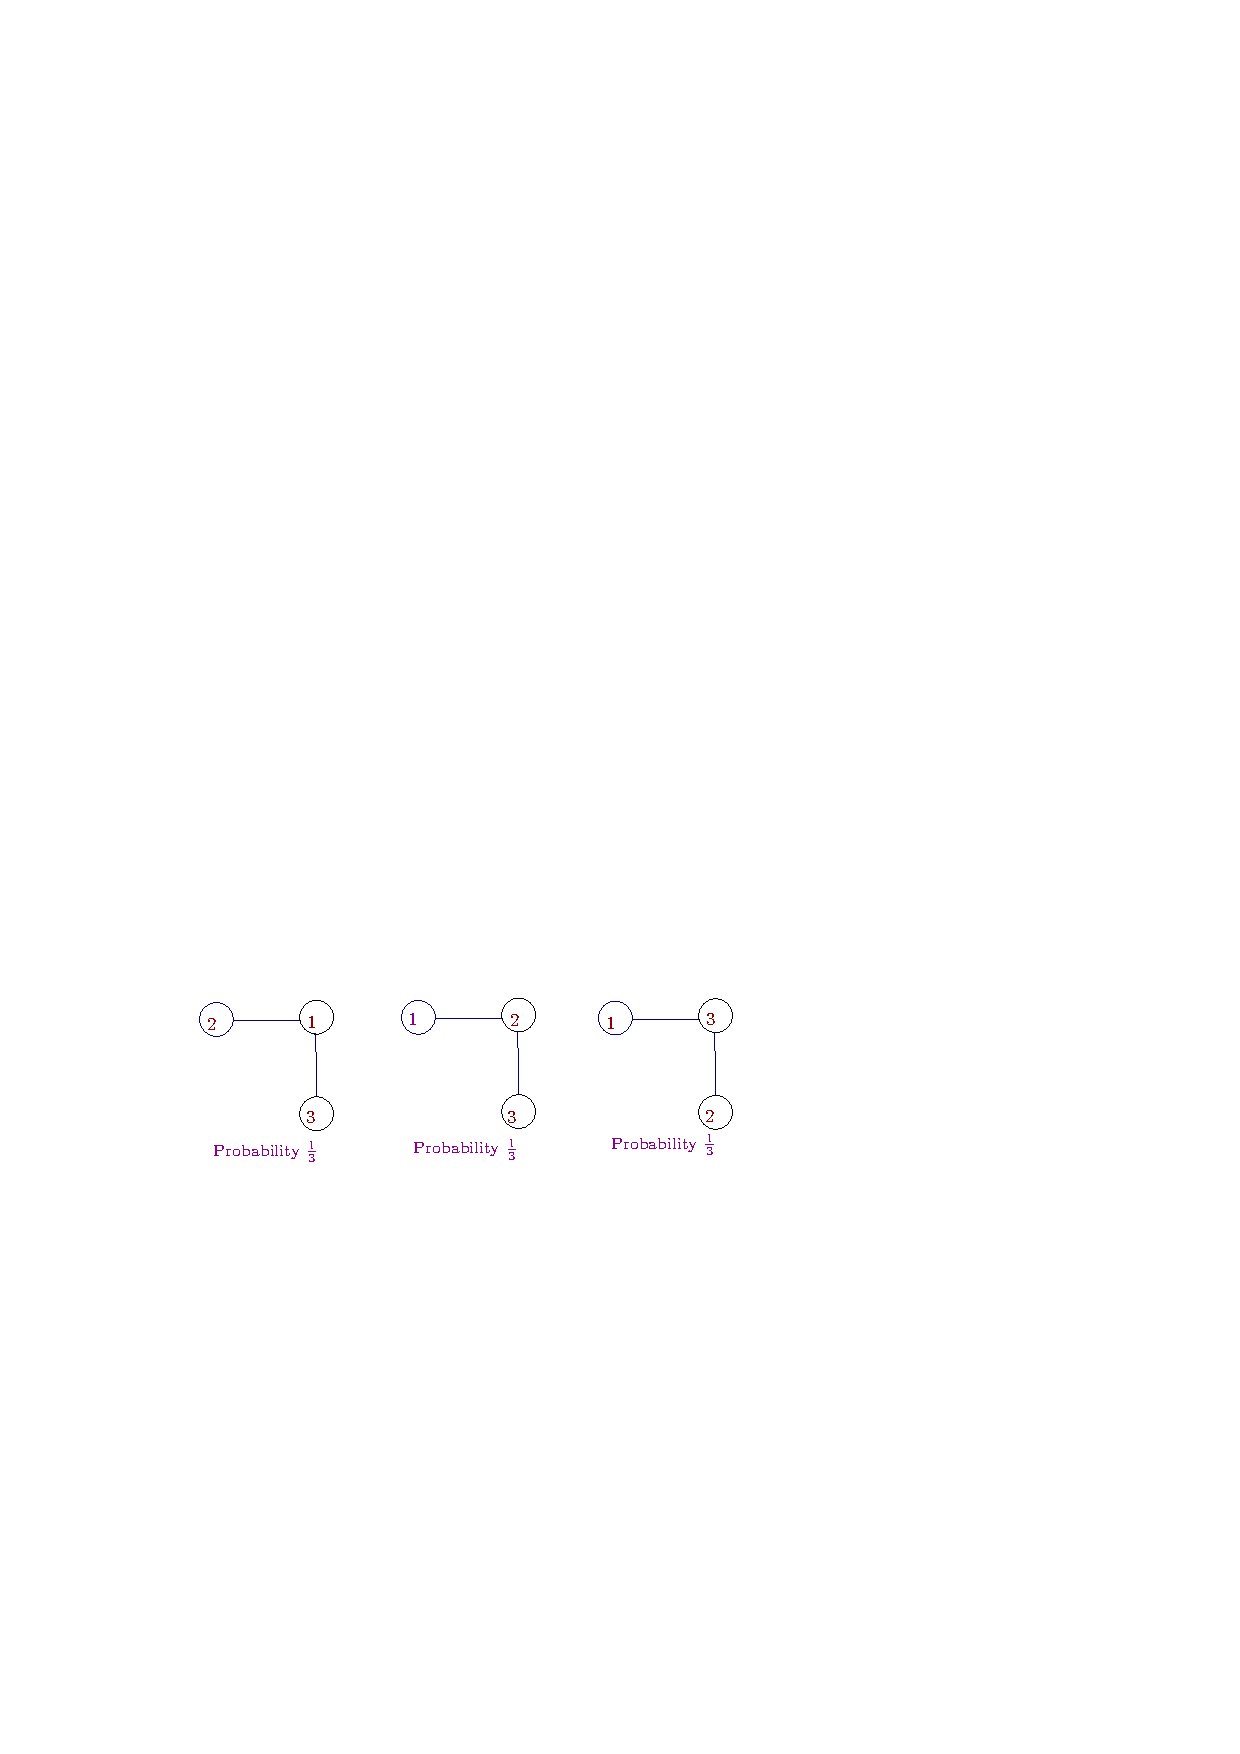
\includegraphics[width=0.8\textwidth]{FIG/random-graph-example} 
\caption{\label{fig:examplerandom} A random graph on $\{1,2,3\}$ with 2 edges with the uniform distribution}
\end{figure*}

\begin{proof}

Consider any graph with $m$ edges, call it $G$. 


\begin{align*} 
\Prob{ G(n,p) = G | |E(G(n,p))|=m} &= \frac{ \Prob{G(n,p)=G} }{\Prob{|E(G(n,p))|=m}} \\ 
                                   &=  \frac{ p^m (1-p)^{    {n \choose 2} - m   }  }{ { {n \choose 2} \choose m } p^m (1-p)^{   {n \choose 2} - m } } \\ 
								   &= \frac{1}{{ {n \choose 2} \choose m }}
\end{align*} 


\end{proof}


\begin{definition}
Define a graph property $\mathcal{P}$ as a subset of all possible labelled graphs. 
Namely $\mathcal{P} \subseteq 2^{[n] \choose 2}$. 
\end{definition} 

For instance $\mathcal{P}$ can be the set of planar graphs or the set of graphs
that contain a Hamiltonian cycle. 
We will call a property $\mathcal{P}$ as monotone increasing if $G \in \mathcal{P}$ 
implies $G+e \in \mathcal{P}$. For instance the Hamiltonian property is monotone 
increasing. 
Similarly, we will call a property $\mathcal{P}$ as monotone decreasing if $G \in \mathcal{P}$ 
implies $G-e \in \mathcal{P}$.
For instance the planarity property is monotone decreasing. 


{\bf Exercise:} Think of other monotone increasing and decreasing properties. 

Consider any monotone increasing property $\mathcal{P}$. Intuitively, the more edges the graph
has, the more likely a random graph has property $\mathcal{P}$\footnote{I will 
use interchangeably the terms a graph {\it has} property $\mathcal{P}$ and a graph 
{\it belongs} in $\mathcal{P}$. }. Indeed, 

\begin{lemma}
\label{lem:lec1lem1}
Suppose $\mathcal{P}$ is a monotone increasing property and $0 \leq p_1 < p_2 \leq 1$. 
Let $G_i \sim G(n,p_i), i=1,2$. Then, 

$$ \Prob{ G_1 \in \mathcal{P} } \leq  \Prob{ G_2 \in \mathcal{P} }.$$
\end{lemma}

\begin{proof}
We will generate $G_2 \sim G(n,p_2)$ from a graph $G_1 \sim G(n,p_1)$.
The idea is called {\it coupling}. After generating $G_1$ we will 
generate a graph $G \sim G(n,p)$ and we will output the union of $G_1 \cup G$
as our $G_2$. We need to choose $p$ in such way that we respect the probability
distributions. To see how to choose $p$ observe the following: 
an edge in $G_2$ does not exist with probability $(1-p_2)$. 
In $G_1 \cup G$ this happens with probability $(1-p)(1-p_1)$. 
By setting 

$$ (1-p_2)=(1-p)(1-p_1)$$ 

\noindent and solving for $p$ we have achieved our goal. 
Given that the property is monotone increasing, we obtain the result. 
\end{proof} 

{\bf Exercise:} Prove an analog lemma for the $G(n,m)$ model. 

Now we prove two facts before we give a general statement for the asymptotic equivalence 
of the two models.

\begin{fact}
Let $\mathcal{P}$ be any graph property, $p=\frac{m}{ {n \choose 2}}$, where $m=m(n), {n \choose 2}-m \rightarrow +\infty$.
Then, asymptotically 


$$ \Prob{ G(n,m) \in \mathcal{P}} \leq \sqrt{ 2 \pi m } \Prob{G(n,p) \in \mathcal{P}}.$$

\end{fact}


\begin{proof}

The probability that we obtain a given graph $G$ depends only on the number of its edges. 
Also notice that there exist ${{n \choose 2} \choose k}$ graphs with $k$ distinct edges, 
for any $0 \leq k \leq {n \choose 2}$. 
Therefore, from the law of total probability we obtain the following expression: 

\begin{align*} 
\Prob{G(n,p) \in \mathcal{P}} &= \sum_{m'=0}^{{n \choose 2}} \Prob{|E(n,p)|=m'} \times \Prob{G(n,p) \in \mathcal{P} | |E(n,p)|=m'} \\ 
                              &\geq \Prob{|E(n,p)|=m} \times \Prob{G(n,p) \in \mathcal{P} | |E(n,p)|=m} \\ 
							   &=\Prob{|E(n,p)|=m} \times \Prob{G(n,m) \in \mathcal{P}}. 
\end{align*}

It suffices to prove that 

$$ \Prob{|E(n,p)|=m} \geq \frac{1}{  \sqrt{ 2 \pi m } }.$$ 

For this purpose we will use Stirling's formula\footnote{Check out 
this post \url{http://gowers.wordpress.com/2008/02/01/removing-the-magic-from-stirlings-formula/} 
for a neat proof by Timothy Gowers.}

$$ n! = (1+o(1)) \sqrt{2 \pi} n^{n+\frac{1}{2}} e^{-n}.$$ 


Also, we observe that the random variable $|E(n,p)|$ is a binomial variable, i.e., $|E(n,p)| \sim Bin( {n \choose 2}, p )$.
Therefore, 

\begin{align*} 
\Prob{|E(n,p)|=m} &= { {n \choose 2} \choose m} p^m (1-p)^{ {n \choose 2} -m} \approx \big ( \frac{ {n \choose 2} }{ 2 \pi m \big({n \choose 2}-m\big)} \big)^{1/2}\\ 
                  &\geq \frac{1}{ \sqrt{ 2 \pi m } }.
\end{align*}
\end{proof}

\noindent {\bf Exercise:} The following fact is left as an exercise. You can solve it either by using the central limit
theorem or by more tedious computations using appropriate asymptotic approximations. 
\begin{fact}
Let $\mathcal{P}$ be a monotonically increasing (decreasing) graph property, 
$p=\frac{m}{ {n \choose 2}}$. 
Then, asymptotically 

$$ \Prob{ G(n,m) \in \mathcal{P}} \leq 3  \Prob{G(n,p) \in \mathcal{P}}.$$

\end{fact}


The following theorem gives precise conditions 
for the asymptotic equivalence of $G(n,p), G(n,m)$ \cite{friezekaronski}, see also \cite{bollobas2001random}. 

\begin{theorem}
Let $0 \leq p_0 \leq 1, s(n) =n \sqrt{p(1-p)} \rightarrow +\infty$, and $\omega(n) \rightarrow +\infty$ 
as $n \rightarrow +\infty$.  Then, 

(a) if $\mathcal{P}$ is any graph property and for all $m \in \field{N}$ such that 
$|m- {n \choose 2}p| <\omega(n)s(n)$, the probability $\Prob{G(n,m) \in \mathcal{P} } \rightarrow p_0$,
then $\Prob{G(n,p) \in \mathcal{P} } \rightarrow p_0$ as $n \rightarrow +\infty$.

(b) if $\mathcal{P}$ is a monotone graph property and $p_{-} = p_0 - \frac{\omega{(n)}s(n)}{n^3}$, 
$p_+ = p_0 +\frac{\omega{(n)}s(n)}{n^3}$ then from the facts that 
$\Prob{ G(n,p_{-}) \in \mathcal{P} } \rightarrow p_0, \Prob{ G(n,p_{+}) \in \mathcal{P} } \rightarrow p_0$,
it follows that $\Prob{ G(n,p{n \choose 2}) \in \mathcal{P} } \rightarrow p_0$ as $n \rightarrow +\infty$.
\end{theorem} 


\subsection{History} 
\label{subsec:lec1unclepaul}

The theory of random graphs was founded  by Paul Erd\"os  and Alfred R\'enyi 
in a series of seminal papers. Erd\"os  and R\'enyi studied 
originally the $G(n,m)$ model. Gilbert proposed the $G(n,p)$ model. 
Some people refer to random binomial graphs as Erd\"os-R\'enyi 
or Erd\"os-R\'enyi-Gilbert. Nonetheless, it was Erd\"os and R\'enyi 
who set the foundations of modern random graph theory. 

Before the series of  Erd\"os-R\'enyi papers, Erd\"os  had discovered that 
the probabilistic method could be used to tackle problems whose statements
were purely deterministic. 
For instance, one of the early uses of random 
graphs was in Ramsey theory. We define the Ramsey number 

$$ R(k,l) = \min \{ n: \forall c:E(K_n)\rightarrow \{\text{red,blue}\} \exists \text{~red~} K_k \text{~or blue~} K_l \}.$$ 

{\bf Example:} Prove $R(3,3)=6$. The next challenge is to show $R(4,4)=18$.

\hide{ 
\noindent Let's consider $R(k,k)$. Another perspective of looking at this number is the following. 
Consider $n$ vertices and take any graph $G$ on $[n]$.  Then either $G$ contains a clique of size 
$k$ or its complement an } 

In one of the next lectures we will study the maximum clique in $G(n,p)$. 
Specifically, by studying  the maximum clique size in $G(n,1/2)$,
we will see why $R(k,k) \geq 2^{k/2}$. Now, let's see a proof based 
on the union bound. 

\begin{theorem}[Erd\"os, 1947] 
$$R(k,k) \geq  2^{k/2}.$$
\end{theorem}

\begin{proof}
Color each edge of the complete graph $K_n$ with red or blue by tossing a fair coin, independently
from the other edges. 
For a fixed subset $S \subseteq [n]$, $|S|=k$ let $A_S$ be the event that $S$ is monochromatic,
i.e., all the ${k \choose 2}$ edges get the same color.
Clearly, $ \Prob{A_S} = 2^{1-{k\choose 2}}$.  Notice that 
if $\Prob{ \cup_{S \subseteq V, |S|=k} A_S} <1$ then the probability 
that none of the $k$-sets is monochromatic is $>0$ which means that 
there exists a 2-coloring which violates the Ramsey property. Hence this would 
suggest that $R(k,k)>n$. 

Based on the union bound

$$ \cup_{S \subseteq V, |S|=k} \Prob{A_S} \leq  {n \choose k} 2^{1-{k \choose 2}}$$ 

\noindent we can deduce that $R(k,k)>n$ if ${n \choose k} 2^{1-{k \choose 2}} <1$. 
When $n=\lfloor 2^{k/2} \rfloor$ then this condition holds. Let's check it. 


$$ {n \choose k} 2^{1-{k \choose 2}} < \frac{n^k}{k!} 2^{1-{k \choose 2}} < 1.$$ 

\end{proof}

%\subsection{Early uses of random graphs: the probabilistic method}
%\label{subsec:lec1earlyuses}

\begin{figure}
  \centering
  {\label{fig:paul}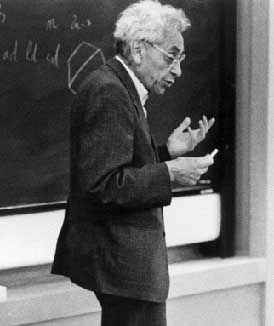
\includegraphics[scale=0.3]{FIG/erdos.jpg}}                
  {\label{fig:alfred}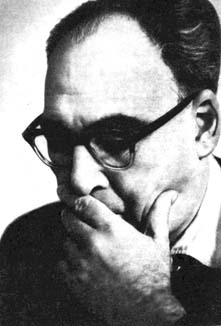
\includegraphics[scale=0.3]{FIG/renyi2.jpg}}
  \caption{Erd\"os  \& R\'enyi, founders of random graph theory }
  \label{fig:erdosrenyi}
\end{figure}


%\subsection{Modern uses of random graphs} 
%\label{subsec:lec1modernuses}

\hide{ 
\section{First and Second Moment Method }

The next two elementary probabilistic tools  are very powerful. Just with these tools, many non-trivial results
can be proved. 


\begin{theorem}[First Moment Method]
\label{thrm:lec1firstmoment} 

Let $X$ a be non-negative integer valued random variable. 
Then, 

$$ \Prob{X > 0 } \leq \Mean{X}.$$ 
\end{theorem} 

Sometimes, it is much easier to compute $\Mean{X}$ than $\Prob{X>0}$. 
Therefore, if we want to prove that $\Prob{X>0}$ tends  to 
0 as $n \rightarrow +\infty$ it suffices to show that $\Mean{X}=o(1)$. 

However, if we want to show that $\Prob{X>0}$ we cannot use the First Moment
Method. The use of the following inequality is also known as Chebyshev's inequality. 

\begin{theorem}[Second Moment Method] 
\label{thrm:lec1secondmoment} 
If X is a nonnegative integer valued random variable then

$$ \Prob{X>0} \geq 1-\frac{ \Var{X}}{ (\Mean{X})^2}.$$ 
\end{theorem}


Typically, Theorem~\ref{thrm:lec1secondmoment}  will do the work. But sometimes
a stronger form of the second moment method is needed. It is stated as the following 
theorem. 

\begin{theorem}[Strong Second Moment Method] 
\label{thrm:lec1strongsecondmoment} 

If X is a nonnegative integer valued random variable then

$$ \Prob{X>0} \geq 1-\frac{ \Var{X}}{ \Mean{X^2}}.$$ 
\end{theorem}


%{\bf Exercise:} Prove Theorems~\ref{thrm:lec1firstmoment}, \ref{thrm:lec1secondmoment} and \ref{thrm:lec1strongsecondmoment}.

}


\section{Thresholds} 

We formalize the notion of a threshold. begin with a formal definition of what we described the previous time.  

\begin{definition}[Threshold] 
A function $p^*=p(n)$ is a threshold for a monotone increasing 
property\footnote{Of course, in the case of monotone decreasing 
properties, the two cases above will be flipped.} $\mathcal{P}$ 
in $G(n,p)$ if 

\[
 \lim_{n \rightarrow +\infty} \Prob{ G(n,p) \in \mathcal{P}}  =
  \begin{cases}
   1       & \text{if } p^*=o(p) (p^* \ll p) \\
   0       & \text{if } p=o(p^*) (p \ll p^*)
  \end{cases}
\]

\noindent as $n \rightarrow +\infty$. 

\end{definition}

Last time, we discussed the existence of thresholds for various monotone properties. 
It is natural to ask whether all monotone properties have a threshold. 
The answer is stated as a theorem without proof. 

\begin{theorem}
Every non-trivial monotone property has a threshold. 
\end{theorem} 

Today, we will discuss two monotone increasing properties, which according to the above theorem 
have a threshold: the appearance of a $K_4$ and connectivity. 
Before we go into the main results of today's class, we will go over 
some basic  tools. 
%We will make use of most of them today, but some of them will be used in future lectures. 

\section{Basic tools: First and Second moment methods}

\hide{ 
We will use the following inequalities to bound the binomial coefficient ${n \choose k}$. 

 \[
 \boxed{ \Big(\frac{n}{k}\Big)^k \leq {n \choose k} \leq \Big(\frac{en}{k}\Big)^k.}
 \]


We will also need to be able to upper- and lower-bound certain expressions.
Here are some useful inequalities. 

  \[
 \boxed{ (1-x)^n \geq 1-nx \text{,~~} \forall  0\leq x \leq 1.}
 \]
 
 \[
 \boxed{  e^x \geq x+1 \text{,~~}\forall x.}
 \]


  \[
 \boxed{  e^x \leq x^2+x+1\text{,~~~} \forall 0<|x|<1.}
 \]

 \[
 \boxed{  \log{(1+x)} = x-\frac{x^2}{2}+ \frac{x^3}{3} - \frac{x^4}{4} +  \ldots \text{,~~~}\forall 0<|x|<1.}
 \]

%Few more important inequalities.

  \[
 \boxed{  \big( \sum_{i=1}^n a_i^2 \big)   \big( \sum_{i=1}^n b_i^2 \big) \geq  \big( \sum_{i=1}^n a_ib_i \big)^2.}
 \]

The above inequality is the Cauchy-Schwartz inequality, which is a special case of H\"older's inequality for $p=q=2$. 

\begin{theorem}[H\"older's inequality]
For any positive real numbers $p,q$ such that $\frac{1}{p}+\frac{1}{q}=1$ 

  \[
 \boxed{  \big( \sum_{i=1}^n |a_i b_i| \big)  \leq   \big( \sum_{i=1}^n |x_i|^p \big)^{1/p}    \big( \sum_{i=1}^n |x_i|^p \big)^{1/p}   .}
 \]
 
\end{theorem} 

}

The next two elementary probabilistic tools  are very powerful. Just with these tools, many non-trivial results
can be proved. 





\begin{theorem}[Markov's Inequality]
\label{thrm:lec1firstmoment} 

Let $X$ a be non-negative integer valued random variable. 
Then, 

$$ \Prob{X \geq t } \leq \frac{\Mean{X}}{t}.$$ 
\end{theorem} 

\begin{proof} 

\begin{align*} 
\Mean{X} &= \sum_{k\geq 1} k \Prob{X=k} \geq \sum_{k=t} k \Prob{X=k} \geq t \sum_{k=t} \Prob{X=k} = t\Prob{X \geq t}.
\end{align*} 

\end{proof}  

We will use this inequality in two ways in our class. First, it is the basis of the first moment
method. In many cases we will need to show that $\Prob{X>0}=o(1)$,  where $X$ is a non-negative 
random variable of interest. It turns out that computing $\Mean{X}$ can be much easier than 
directly computing $\Prob{X>0}$  in numerous
cases. 
If $\Mean{X}=o(1)$ then by Markov's inequality

 \[
 \boxed{\Prob{X>0}\leq \Mean{X}}
 \]
 
\noindent we obtain that $X=0$ \whp.  This use is known as the {\em first moment method}. 
Furthermore, we will use Markov's inequality to obtain probabilistic inequalities 
for higher order moments.  This is a special case of the following observation. 
If $\phi$ is a strictly monotonically increasing function, then 

$$ \Prob{ X \geq t} = \Prob{\phi(X) \geq \phi(t) } \leq \frac{ \Mean{ \phi(X) } }{\phi(t)}.$$ 

For instance, if $\phi(x)=x^2$, then we obtain Chebyshev's inequality. 

\begin{theorem}[Chebyshev's Inequality] 
Let $X$ be {\it any} random variable. Then,
$$ \Prob{ |X-\Mean{X}| \geq t} \leq \frac{\Var{X}}{t^2}.$$
\end{theorem}


A simple corollary of Chebyshev's inequality   
is the following: 

\begin{corollary}[Second moment method] 
Let $X$ be a non-negative integer valued random variable. Then, 

 \[
 \boxed{\Prob{X=0} \leq \frac{ \Var{X} } { (\Mean{X})^2 }.}
 \]
 
 
\end{corollary}

For completeness, here is the proof.

\begin{proof}
$$\Prob{X = 0}  \leq \Prob{ |X - \Mean{X}| \geq \Mean{X} } \leq \frac{ \Var{X} }{ (\Mean{X})^2 }.$$
\end{proof}


The use of the above corollary is known as the second moment method. 
Here is how we will typically use it in our class. 
Let the random variable $X$ of interest be the sum of $m$ indicator
random variables $X_1,\ldots,X_m$, where $\Prob{X_i=1}=p_i$, i.e.,

$$ X = X_1 + \ldots + X_m.$$ 

\noindent We will be interested in showing that $X>0$ \whp. 
Even if $\Mean{X}$ will tend to $+\infty$ this does not suggest 
that $X>0$ \whp. 
In order to prove this kind of statement, we will 
use the second moment method. Since $\Prob{X = 0}  \leq   \frac{ \Var{X} }{ (\Mean{X})^2 }$
it will suffice to prove that $  \frac{ \Var{X} }{ (\Mean{X})^2 } = o(1)$.  
The problem therefore is reduced to computing or actually {\em upper-bounding} the variance. 

In our typical setting, 

$$ \Var{X} = \sum_{i=1}^m \Var{X_i} + \sum_{i \neq j} \Cov{ X_i,X_j} \leq \Mean{X} + \sum_{i \neq j} \Cov{X_i,X_j} .$$ 

To see how we obtained the inequality, notice that $\Var{X_i} = p_i(1-p_i) \leq p_i = \Mean{X_i}$.
Hence by the linearity of expectation $\sum_i \Var{X_i} \leq \sum_i \Mean{X_i}=\Mean{X}$. 
The covariance of two random variables $A,B$ is defined as 

$$ \Cov{A,B} = \Mean{AB} - \Mean{A}\Mean{B}.$$ 

In the case of indicator random variables we obtain the following expression: 

$$ \Cov{X_i,X_j} = \Prob{ X_i = X_j =1 } - \Prob{X_i=1} \Prob{X_j=1}.$$ 

So, when we apply the second moment, the hard part it to upper bound the sum of covariances. 
Section~\ref{sec:lec2emergenceH} illustrates a use of the first and second moment methods. 

\section{Emergence of a $K_4$ in $G(n,p)$}%a fixed subgraph $H$} 
\label{sec:lec2emergenceH} 


A $K_4$ is a complete graph on four vertices.  Let $X$ be the number of $K_4$s in $G(n,p)$. 
We will show that the threshold value $p^*$ is equal to $n^{-2/3}$. 
%First, let's see how heuristically we can find such threshold values. 
The expectation of $X$ 

$$ \Mean{X} = {n \choose 4} p^6.\footnote{The number of edges in $K_4$ is ${4 \choose 2}=6$.}$$

\noindent Let's see what happens to $\Mean{X}$ if $p \ll p^*$ or equivalently $p=\frac{p^*}{\omega(n)}$ where 
$\omega(n)$ is a function that tends to $+\infty$ as $n \rightarrow +\infty$. 

$$ \Mean{X} = {n \choose 4} p^6 = \Theta\Bigg(n^4 \Big(\frac{n^{-2/3}}{\omega(n)}\Big)^6\Bigg) = \Theta\Bigg( \frac{1}{ \big( \omega(n)\big)^6}\Bigg)=o(1).$$

Hence by the first moment method we can conclude that when $p \ll n^{-2/3}$ 

$$ \Prob{X>0} \leq \Mean{X} = o(1),$$ 

\noindent or equivalently $X=0$ \whp. 
Now, we will prove that $X>0$ \whp when $p^* \ll p$ or equivalently $p=p^*\omega(n)$ where 
$\omega(n)$ is a function that tends to $+\infty$ as $n \rightarrow +\infty$. 
Notice now that the expected value of K4s goes to infinity, namely 

$$ \Mean{X} = {n \choose 4} p^6 = \Theta\Bigg(n^4 \big( n^{-2/3}\omega(n)\big)^6\Bigg) = \Theta\Bigg( (\omega(n))^6\Bigg) \rightarrow +\infty.$$


\noindent However, this does not suggest that $X>0$ \whp. We need to apply the second moment method. 
First, let's define an indicator variable $X_i$ for the $i$-th labeled copy of $K_4$ in $K_n$, 
$i=1,\ldots,{n \choose 4}$. We can write

$$ X = X_1 + X_2 + \ldots + X_{{n \choose 4}}.$$ 

What is the covariance of two indicator variables here? Well, let's see how dependencies
kick in. When two copies of $K_4$ share no edge then the respective indicator variables 
are independent. To see why observe that  in this case 

 
$$ \Cov{X_i, X_j} = \Prob{X_i=X_j=1} - \Prob{X_i}\Prob{X_j} = p^{12}-p^6p^6=0.$$

Equivalently, for the case of $K_4$ this happens if two $K_4$ copies intersect in 0 or 1 vertex. 
We are left with two cases, which are shown in figure~\ref{fig:lec2k4s}. 
Let's consider the covariance for case (a). 
What is the probability that the two indicator variables are both 1? 
Since the two copies have two vertices in common, or equivalently 1 edge, 
the total number of edges is $11$. Hence we get that the covariance is 

$$ \Cov{X_i,X_j} = p^{11}-p^{12}.$$ 

\noindent Similarly, for case (b), we obtain that 

$$ \Cov{X_i,X_j} = p^9-p^{12}.$$ 

Now we have to count how many pairs of indicator variables fall into case (a)
and case (b). In case (a) we have ${n \choose 6}$ ways to choose 6  
out of $n$ vertices and ${6 \choose 2,2,2}$ ways to choose the specific 
labeled configuration. Similarly for case (b), we have ${n \choose 5}  {5 \choose 3,1,1}$
such pairs of indicator variables. Putting everything together gives

$$ \Var{X} \leq {n \choose 4}p^6+ {n \choose 6} {6 \choose 2,2,2} p^{11} + {n \choose 5}  {5 \choose 3,1,1} p^9=o(n^8p^{12})=o\big( (\Mean{X})^2\big).$$

\noindent This concludes the proof that $X>0$ \whp when $p^* \ll p$. 

 
\begin{figure}
	\centering
	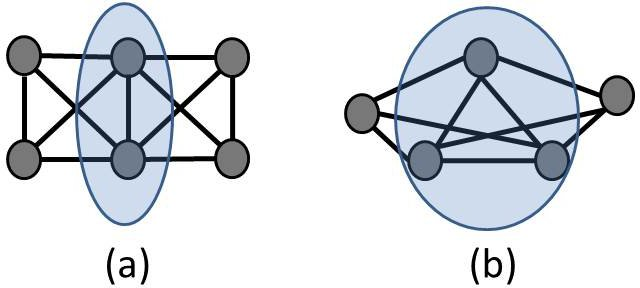
\includegraphics[width=0.5\textwidth]{FIG/k4s} 
	\caption{\label{fig:lec2k4s} The two cases we need to consider in the covariance estimation for $K_4$s.
	Intersections of the two copies are highlighted with a shaded blue area. }
\end{figure}


\section{More on Random Graphs}

Here is a list of textbooks and other resources on random graphs. 

\begin{itemize} 
	\item \txtmagenta{ Random graphs, by {\it B{\'e}la Bollob{\'a}s} \cite{bollobas2001random}}
	\item \txtmagenta{ Complex graphs and networks, by  {\it Fan Chung Graham and  Linyuan Lu} \cite{chung2006complex}}
	\item Random graphs, by {\it Svante Janson, Tomasz Luczak and Andrzej Rucinski} \cite{janson2000random}
	\item \txtmagenta{ Random Graph Dynamics, by {\it Rick Durrett} \cite{durrett2007random} }
	\item Random Graphs and Complex Networks, by {\it Remco Van Der Hofstad} 
	available online at \url{http://www.win.tue.nl/~rhofstad/NotesRGCN2013.pdf}
    \item  Networks, Crowds, and Markets: Reasoning About a Highly Connected World, by {\it David Easley and Jon Kleinberg}
	available online at \url{http://www.cs.cornell.edu/home/kleinber/networks-book/} 
    \item \txtmagenta{ Alan Frieze's notes, available online at \url{http://www.math.cmu.edu/~af1p/Teaching/RandomGraphs/RandomGraphs.html}}
\item \txtmagenta{The Probabilistic Method by {\it Noga Alon and Joel Spencer} \cite{noga}.}
\end{itemize} 

\bibliographystyle{sapalike}
\bibliography{lecref}

\end{document}





